\section{Sensores}
Los sensores son dispositivos que permiten a los robots percibir su entorno y obtener información sobre su posición, movimiento, temperatura, proximidad, presión, entre otros aspectos. Estos sensores convierten datos físicos en señales eléctricas que el robot puede procesar para tomar decisiones o realizar tareas.

Se clasifican en:

	\subsection{Sensores Externos}
		\begin{enumerate}
			\item \textbf{Posición}
			\begin{enumerate}
				\item Lineal
				\item Rotativo
			\end{enumerate}
			
			\item \textbf{Velocidad}
			\begin{enumerate}
				\item Todos los sensores de posición
				\item Tacómetro
				\item Sensor de efecto Hall
			\end{enumerate}
			
			\item \textbf{Aceleración}
			\begin{enumerate}
				\item Todos los sensores de fuerza
			\end{enumerate}
			
			\item \textbf{Fuerza}
			\begin{enumerate}
				\item Galgas extensométricas
				\item Interruptores de límite
				\item Interruptores piezoeléctricos
			\end{enumerate}
		\end{enumerate}
		
	\subsection{Sensores Internos}
	 \begin{enumerate}
		\item \textbf{Tipo de contacto}
		\begin{enumerate}
			\item Interruptores de límite
			\item Interruptores neumáticos
			\item Sensores piezoeléctricos
			\item Transductores de presión
		\end{enumerate}
		\item \textbf{Tipo sin contacto}
		\begin{enumerate}
			\item Sensores de proximidad
			\item Sensores de efecto Hall
			\item Sensores de microondas
			\item Sensores ultrasónicos
			\item Sensores láser
			\item Sensores de visión
		\end{enumerate}
	\end{enumerate}

Para usar dos imágenes como en \autoref{fig:mascotas}, se utilizó \texttt{subfloat}.
% Dos imágenes de mascotas
\begin{figure}[h]
	\centering
	\subfloat[Perro]{%
		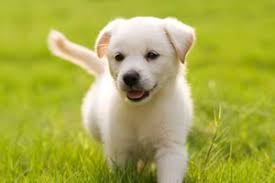
\includegraphics[width=0.4\textwidth]{perro.jpg}%
		\label{fig:perro}
	}
	\hfill
	\subfloat[Gato]{%
		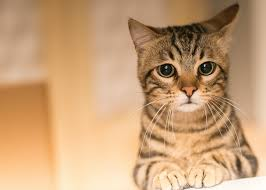
\includegraphics[width=0.4\textwidth]{gato.jpg}%
		\label{fig:gato}
	}
	\caption{Imagen de dos mascotas}
	\label{fig:mascotas}
\end{figure}